\documentclass[extra,mreferee]{gji}
% Use the option below to make a nicely formatted manuscript
%\documentclass[extra]{gji}

\usepackage{timet}
\usepackage{graphicx}

\title[Optimal forward modeling using tesseroids]{
    Optimal forward modeling of gravitational fields
    using tesseroids with adaptive discretization
}
\author[Uieda et al.]{
    Leonardo Uieda$^{1,2}$,
    Vanderlei C. Oliveira Jr$^2$,
    Val\'eria C. F. Barbosa$^2$
    \\
    $^1$Universidade do Estado do Rio de Janeiro, Rio de Janeiro, Brazil.
    $^2$Observat\'orio Nacional, Rio de Janeiro, Brazil.
}

\begin{document}

\label{firstpage}
\maketitle


\begin{summary}
Lorem ipsum dolor sit amet, consectetur adipiscing elit. Nam eu dolor pretium,
egestas mauris sed, dapibus quam. Duis hendrerit mollis nunc a consequat. Nulla
et sem consectetur, interdum velit eget, aliquam ipsum. Praesent sagittis
tortor diam, sed ultrices magna ullamcorper vitae. Proin vitae orci augue.
Morbi dictum ligula gravida sem malesuada facilisis. Mauris nibh metus, cursus
eget imperdiet vitae, pretium at lorem. Praesent nisi mauris, pretium ut risus
fermentum, egestas tincidunt nibh. Mauris nulla orci, consequat eu pharetra
non, mattis ut urna. Mauris facilisis orci eros. Nam mattis non magna iaculis
consectetur. Morbi sodales dolor vitae felis sagittis, eget faucibus turpis
convallis. Nullam malesuada, mauris et ultricies rutrum, odio nulla gravida
nunc, ac volutpat eros lectus eget lacus. Integer venenatis velit vel justo
pellentesque, quis molestie sem vestibulum.
\end{summary}

%%%%%%%%%%%%%%%%%%%%%%%%%%%%%%%%%%%%%%%%%%%%%%%%%%%%%%%%%%%%%%%%%%%%%%%%%%%%%%
\section{Introduction}

Citing articles in text \citet{Asgharzadeh2007} and with parenthesis
\citep{Braitenberg2011}.

The above integrals
have to be solved numerically
\citep{Wild-Pfeiffer2008}
and different approaches have been proposed in the literature.
\citet{Heck2007}
used a Taylor series expansion
of the integral kernels
around the geometrical center of the tesseroid.
\citet{Asgharzadeh2007}
used the Gauss-Legendre Quadrature (GLQ)
for the numerical integration.
\citet{Wild-Pfeiffer2008} investigated
the use of both methods,
along with alternative mass elements,
and found the GLQ to be the most efficient method.
We have opted to use
the 3D GLQ integration in our computations.

The accuracy of the numerical integration
using the GLQ
was investigated by \citet{Ku1977}
for the case of
the gravitational attraction of
a right-rectangular prism
in Cartesian coordinates.
\citet{Ku1977} states that the accuracy
depends on the ratio between
the average distance between GLQ nodes
and the distance to the observation point P.
As a rule-of-thumb,
\citet{Ku1977} suggests that
the distance between nodes
should not be greater than
the distance to point P.
Extrapolating this rule-of-thumb
to tesseroids,
\citet{Li2011}
devised a scheme that
recursively divides a tesseroid
into smaller ones when the rule is violated.
This procedure
effectively decreases the distance between nodes
and, theoretically, guarantees the accuracy of the GLQ integration.

%%%%%%%%%%%%%%%%%%%%%%%%%%%%%%%%%%%%%%%%%%%%%%%%%%%%%%%%%%%%%%%%%%%%%%%%%%%%%%
\section{Methodology}

The gravitational potential,
gravitational acceleration,
and Marussi (gravity gradient) tensor
caused by a homogeneous tesseroid
with density $\rho$
are \citep{Grombein2013}

\begin{equation}
    V(r,\phi,\lambda) = G \rho
        \int\limits_{\lambda_1}^{\lambda_2}
        \int\limits_{\phi_1}^{\phi_2}
        \int\limits_{r_1}^{r_2}
        \frac{1}{\ell} \kappa  dr' d\phi' d\lambda',
    \label{eq:tesspot}
\end{equation}
\begin{equation}
    g_{\alpha}(r,\phi,\lambda) = G \rho
        \int\limits_{\lambda_1}^{\lambda_2}
        \int\limits_{\phi_1}^{\phi_2}
        \int\limits_{r_1}^{r_2}
        \frac{\Delta_{\alpha}}{\ell^3} \kappa dr' d\phi' d\lambda'
        \ \ \ \alpha \in \{x,y,z\},
    \label{eq:tessgrav}
\end{equation}

\noindent
and

\begin{equation}
    g_{\alpha\beta}(r,\phi,\lambda) = G \rho
        \int\limits_{\lambda_1}^{\lambda_2}
        \int\limits_{\phi_1}^{\phi_2}
        \int\limits_{r_1}^{r_2}
        I_{\alpha\beta}
        dr' d\phi' d\lambda',
    \label{eq:tesstensor}
\end{equation}

\noindent
in which
$(\phi, \lambda, r)$ are
the latitude, longitude, and radius
coordinates of computation point P (Fig.~\ref{fig:tesseroid}),
$\alpha,\beta \in \{x,y,z\}$
are the local coordinate system of point P,
and

\begin{eqnarray}
    I_{\alpha\beta} &=&
        \left(
            \frac{3\Delta_{\alpha} \Delta_{\beta}}{\ell^5} -
            \frac{\delta_{\alpha\beta}}{\ell^3}
        \right) \kappa, \\
    \Delta_x &=& r' K_{\phi} , \\
    \Delta_y &=& r' \cos \phi' \sin(\lambda' - \lambda) , \\
    \Delta_z &=& r' \cos \psi - r, \\
    \ell &=& \sqrt{r'^2 + r^2 - 2 r' r \cos \psi} , \\
    \cos\psi &=& \sin\phi\sin\phi' + \cos\phi\cos\phi'
                 \cos(\lambda' - \lambda) , \\
    K_{\phi} &=& \cos\phi\sin\phi' - \sin\phi\cos\phi'
                 \cos(\lambda' - \lambda), \\
    \kappa &=& {r'}^2 \cos \phi'.
\end{eqnarray}

\noindent
$\delta_{\alpha\beta}$ is the Kronecker delta,
i.e. $\delta_{\alpha\beta}=1$ if $\alpha=\beta$
and $\delta_{\alpha\beta}=0$ otherwise.

\begin{figure}
    \centering
    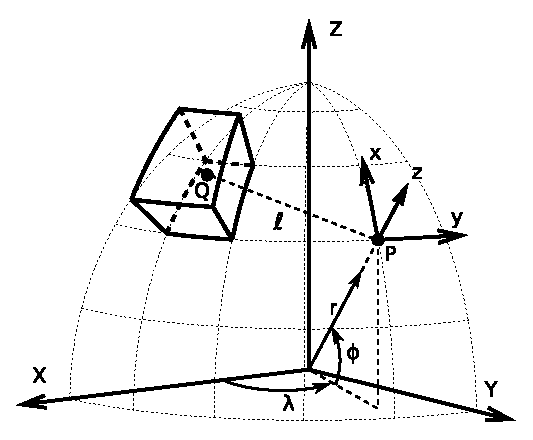
\includegraphics{figs/tesseroid}
    \caption{
        View of a tesseroid,
        the integration point $Q$ inside the tesseroid,
        a geocentric coordinate system $(X, Y, Z)$,
        the computation $P$ and it's local coordinate system $(x, y, z)$.
        $r$, $\phi$, $\lambda$ are
        the radius, latitude, and longitude, respectively, of point $P$,
        and $\ell$ is the Cartesian distance between $P$ and $Q$.
    }
    \label{fig:tesseroid}
\end{figure}

We have opted to use
the 3D Gauss-Legendre Quadrature
to numerically integrate
\ref{eq:tesspot},
\ref{eq:tessgrav},
and
\ref{eq:tesstensor}.
The GLQ
approximates the integral by
a weighted sum
\citep{Hildebrand1987},
e.g.

\begin{equation}
    \int\limits_a^b f(x) dx \approx
    \frac{b-a}{2}\sum\limits_{i=1}^N W_i f(x_i),
\end{equation}

\noindent
where
$W_i$ are weights and
the discretization points (nodes) $x_i$
are the roots of the $N$th order Legendre polynomial $P_N$
scaled to the integration limits.
The roots of a second-order Legendre polynomial are
$x_1=-0.577350269$ and $x_2=0.577350269$.
For an arbitrary order $N$,
we have used the root-finder algorithm
of \citet{Barrera-Figueroa2006}
to calculate the roots of $P_N$.
The weights $W_i$ are \citep{Hildebrand1987}

\begin{equation}
    W_i = \frac{2}{(1 - x_i^2)(P'_N(x_i))^2},
\end{equation}

\noindent
where $P'_N$ is the first derivative of $P_N$.

The triple integrals in equations
\ref{eq:tesspot},
\ref{eq:tessgrav},
and
\ref{eq:tesstensor}
become

\begin{equation}
    V(r,\phi,\lambda) \approx
        A
        \sum\limits_{k=1}^{N^{\lambda}}
        \sum\limits_{j=1}^{N^{\phi}}
        \sum\limits_{i=1}^{N^r}
        W^r_i W^{\phi}_j W^{\lambda}_k
        \frac{1}{\ell} \kappa,
\end{equation}
\begin{equation}
    g_{\alpha}(r,\phi,\lambda) \approx
        A
        \sum\limits_{k=1}^{N^{\lambda}}
        \sum\limits_{j=1}^{N^{\phi}}
        \sum\limits_{i=1}^{N^r}
        W^r_i W^{\phi}_j W^{\lambda}_k
        \frac{\Delta_{\alpha}}{\ell^3} \kappa,
\end{equation}

\noindent
and

\begin{equation}
    g_{\alpha\beta}(r,\phi,\lambda) \approx
        A
        \sum\limits_{k=1}^{N^{\lambda}}
        \sum\limits_{j=1}^{N^{\phi}}
        \sum\limits_{i=1}^{N^r}
        W^r_i W^{\phi}_j W^{\lambda}_k
        I_{\alpha\beta},
\end{equation}

\noindent
where

\begin{equation}
    A = G \rho
    \frac{(\lambda_2 - \lambda_1)(\phi_2 - \phi_1)(r_2 - r_1)}{8},
\end{equation}

\noindent
$W_i^r$, $W_j^{\phi}$, and $W_k^{\lambda}$
are the weights
and $N^r$, $N^{\phi}$, and $N^{\lambda}$
are the number of nodes
for the radial, latitudinal, and longitudinal dimensions, respectively.

The accuracy of the integration
depends on the number of nodes, or GLQ order,
used in the discretization.
However, \citet{Ku1977} showed
that it also depends on the ratio between
the distance to the computation point
and the distance between adjacent nodes.
Fig.~\ref{fig:sample}
illustrates this effect.
To increase the accuracy of the integration,
one could increase the number of nodes,
as in Fig.~\ref{fig:sample}c.
Likewise,
one could keep the number of nodes fixed
and instead divide the tesseroid into smaller ones.
This would increase the total number of nodes
and effectively decrease
the distance between adjacent nodes.
The latter is the approach
taken by \citet{Li2011}.
Here, we will follow the same approach
and make some improvements to the algorithm.
We will also attempt to quantify
the error committed in the numerical integration.

\begin{figure*}
    \centering
    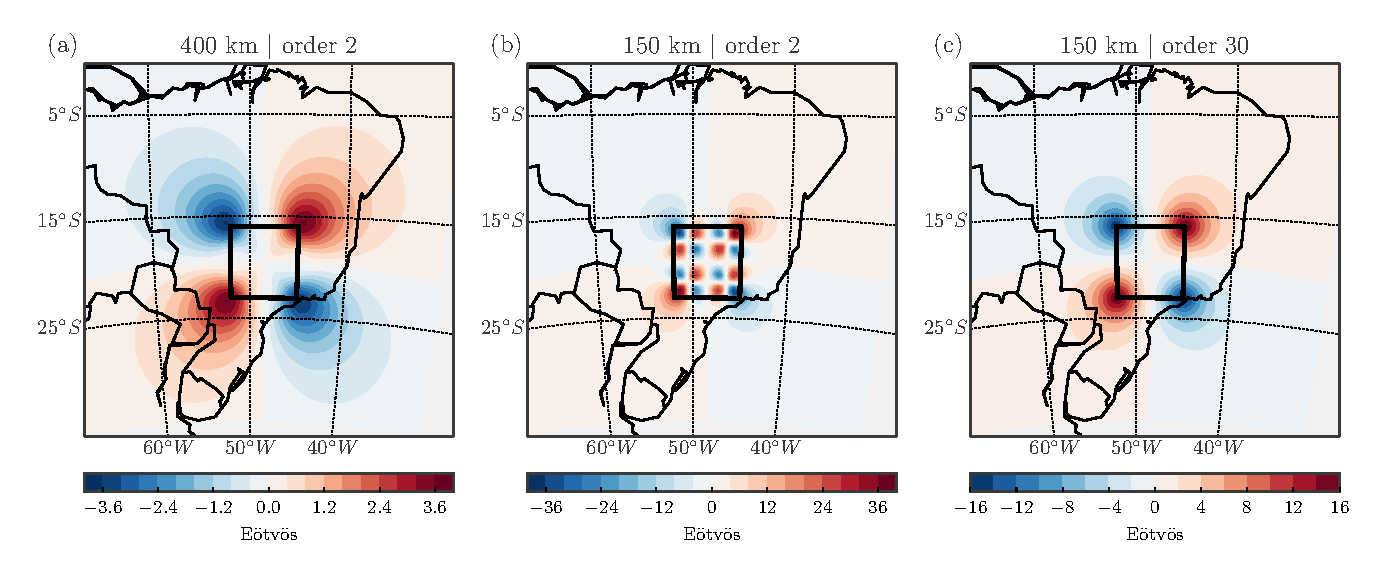
\includegraphics[width=\textwidth]{figs/vary-height-and-order}
    \caption{
        Example of the effect of varying
        the computation height and the Gauss-Legendre Quadrature order
        (number of nodes in each dimension).
        The $g_{xy}$ component caused by a
        $7^\circ \times 7^\circ \times 20\ km$ tesseroid
        with $2.67\ g.cm^{-3}$ density
        and top at $z=0$
        was calculated on a regular grid
        at different heights and using different orders.
        The GLQ order used was the same for all three dimensions.
        a) At $400\ km$ height and order 2, the effect is similar to that
        presented by \citet{Asgharzadeh2007}. b) At $150\ km$ height and order
        2, the effect resembles that of four point sources located at the GLQ
        nodes. c) At $150\ km$ but with a higher order of 30, the effect is
        again similar to the maps in \citet{Asgharzadeh2007}.
    }
    \label{fig:sample}
\end{figure*}

\subsection{Recursive division algorithm}

We have developed a modified version
of the recursive division algorithm of \citet{Li2011}.
We fix the number of nodes in the GLQ
$N^\lambda=N^\phi=N^r=2$
so that the distance between nodes
in the radial, longitudinal, and latitudinal directions
are approximately the dimensions of the tesseroid
\citep{Wild-Pfeiffer2008}.
We define the distance $d$ as
the Cartesian distance between
the computation point $P$
and the center of the top face of the tesseroid
(Fig.~\ref{fig:ratio}a).

DESCRIBE ALGORITHM FIRST.

Thus, the rule-of-thumb of \citet{Ku1977}
can be interpreted as

\begin{equation}
    \frac{d}{L_\zeta} < r,
    \label{eq:ratio}
\end{equation}

\noindent
where
$L_\zeta$, $\zeta \in \{r, \phi, \lambda\}$,
is one of the dimensions of the tesseroid
and
$r$ is the maximum allowed ratio between distance and size.
For \citet{Ku1977}, this ratio should be equal to one.
The dimensions of the tesseroid are

\begin{eqnarray*}
    L_r &=& r_2 - r_1,\\
    L_\phi &=& R(\phi_2 - \phi_1),\\
    L_\lambda &=& R(\lambda_2 - \lambda_1),
\end{eqnarray*}

\noindent
where $R$ is the mean Earth radius
and the longitudes and latitudes are given in radians.

In case the tesseroid is divided,
the inequality in equation \ref{eq:ratio}
is checked for each of the eight parts.
This process is repeated recursively
until no divisions are required,
ensuring that equation \ref{eq:ratio}
holds for all tesseroids created.
The gravitational effect
of the original tesseroid
is then calculated as
the sum of the effect
of the smaller tesseroids.

\begin{figure}
    \centering
    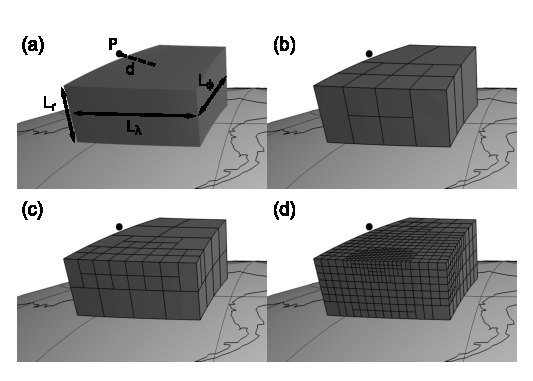
\includegraphics{figs/tesseroid-split}
    \caption{
        Adaptive discretization
        of the tesseroid shown in (a)
        for a computation point P
        using $R$ equal to
        (b) 1, (c) 2, and (d) 6.
        $d$ is the distance between
        the center of the top face of the tesseroid
        and $P$.
        $L_r$, $L_\phi$, and $L_\lambda$ are the dimensions of the tesseroid.
    }
    \label{fig:ratio}
\end{figure}

The rule-of-thumb of \citet{Ku1977}
used by \citet{Li2011}
is equivalent to setting $R=1$.
Fig.~\ref{fig:ratio}
illustrates the subdivision of a tesseroid
(Fig.~\ref{fig:ratio}a)
for computation point $P$
using increasing values of $R$.
Note that increasing $R$
results is a finer division of the tesseroid
around the computation point
and thus a more accurate GLQ integration.
However, higher values of $R$
also result in
larger computation times.
For example,
the tesseroid in Fig.~\ref{fig:ratio}a
is replaced by
50 tesseroids for $R=0.5$ (Fig.~\ref{fig:ratio}b),
344 tesseroids for $R=1$ (Fig.~\ref{fig:ratio}c),
and 2472 tesseroids for  $R=2$ (Fig.~\ref{fig:ratio}d).

Clearly,
there is need to determine
an optimal value of $R$
that yields the desired accuracy
in the GLQ integration.
In the following section,
we compare the computed gravitational effects
of a tesseroid model
with that of a spherical half-shell
for which exist analytical expressions.


\subsection{Determination of $r$ by comparison with a spherical shell}

The gravitational potential,
gravitational attraction,
and
Marussi (gravity gradient) tensor
caused by the homogeneous spherical half-shell
at a computation point
$P = (\lambda=90^\circ, \phi=0^\circ, r=r_2+h)$
are

\begin{equation}
    V(h) = 2\pi G \rho \left[
        \frac{l^3 + {r'}^3}{3(r_2 + h)} - 0.5 {r'}^2 \right]
         \Biggr|_{r'=r_1}^{r'=r_2},
    \label{eq:shellpot}
\end{equation}
\begin{equation}
    g_z(h) = 2\pi G \rho \left[
        \frac{l^3 + {r'}^3}{3(r_2 + h)^2} - l \right]
        \Biggr|_{r'=r_1}^{r'=r_2},
    \label{eq:shellgz}
\end{equation}
\begin{equation}
    g_{xx}(h) = g_{yy}(h) = -\frac{1}{2} g_{zz}(h),
\end{equation}
\begin{equation}
    g_{xy}(h) = g_{xz}(h) = g_{yz}(h) = 0,
\end{equation}

\noindent
and

\begin{equation}
    g_{zz}(h) = 2\pi G \rho \left[
        2\frac{l^3 + {r'}^3}{3(r_2 + h)^3}
        - \frac{l}{r_2 + h} + \frac{r_2 + h}{l}
        \right]
        \Biggr|_{r'=r_1}^{r'=r_2},
    \label{eq:shellgzz}
\end{equation}

\noindent
where $\rho$ is the density,
$l = \sqrt{(r_2 + h)^2 + {r'}^2}$,
and
$r_1$ and $r_2$ are radial coordinates of
the bottom and top of the spherical shell,
respectively.

For our comparison,
we used a spherical half-shell with
$\rho=2.7\ g.cm^{-3}$,
$r_1=6378.137\ km$ (mean Earth radius),
and
$r_2 = r_1 + 50\ km$.
We discretized the half-shell
into tesseroids of equal size
and calculated the gravitational effects of
the half-shell
(using equations \ref{eq:shellpot}-\ref{eq:shellgzz})
and the corresponding tesseroid model
at various heights.
These calculations were repeated
for varying values of
the distance/size ratio $R$.
This analysis
allows us to establish
the optimal value of $R$
that achieves a desired error level.

Data and source code to produce the results of this comparison
are provided by \textbf{(cite notebook on figshare)}.

\subsection{Software implementation}

The methods described above
were implemented the software package
Tesseroids version 1.1.1.
The package consists
of a range of command-line programs
written in the C programming language.
It is freely available
online\footnote{www.leouieda.com/tesseroids}
under the terms of
the open-source BSD 3-clause license.
\textbf{(cite archive on figshare)} provides a persistent
archive for the source code and compiled binaries of Tesseroids.


%%%%%%%%%%%%%%%%%%%%%%%%%%%%%%%%%%%%%%%%%%%%%%%%%%%%%%%%%%%%%%%%%%%%%%%%%%%%%%
\section{Results}

Meh.

\begin{figure*}
    \centering
    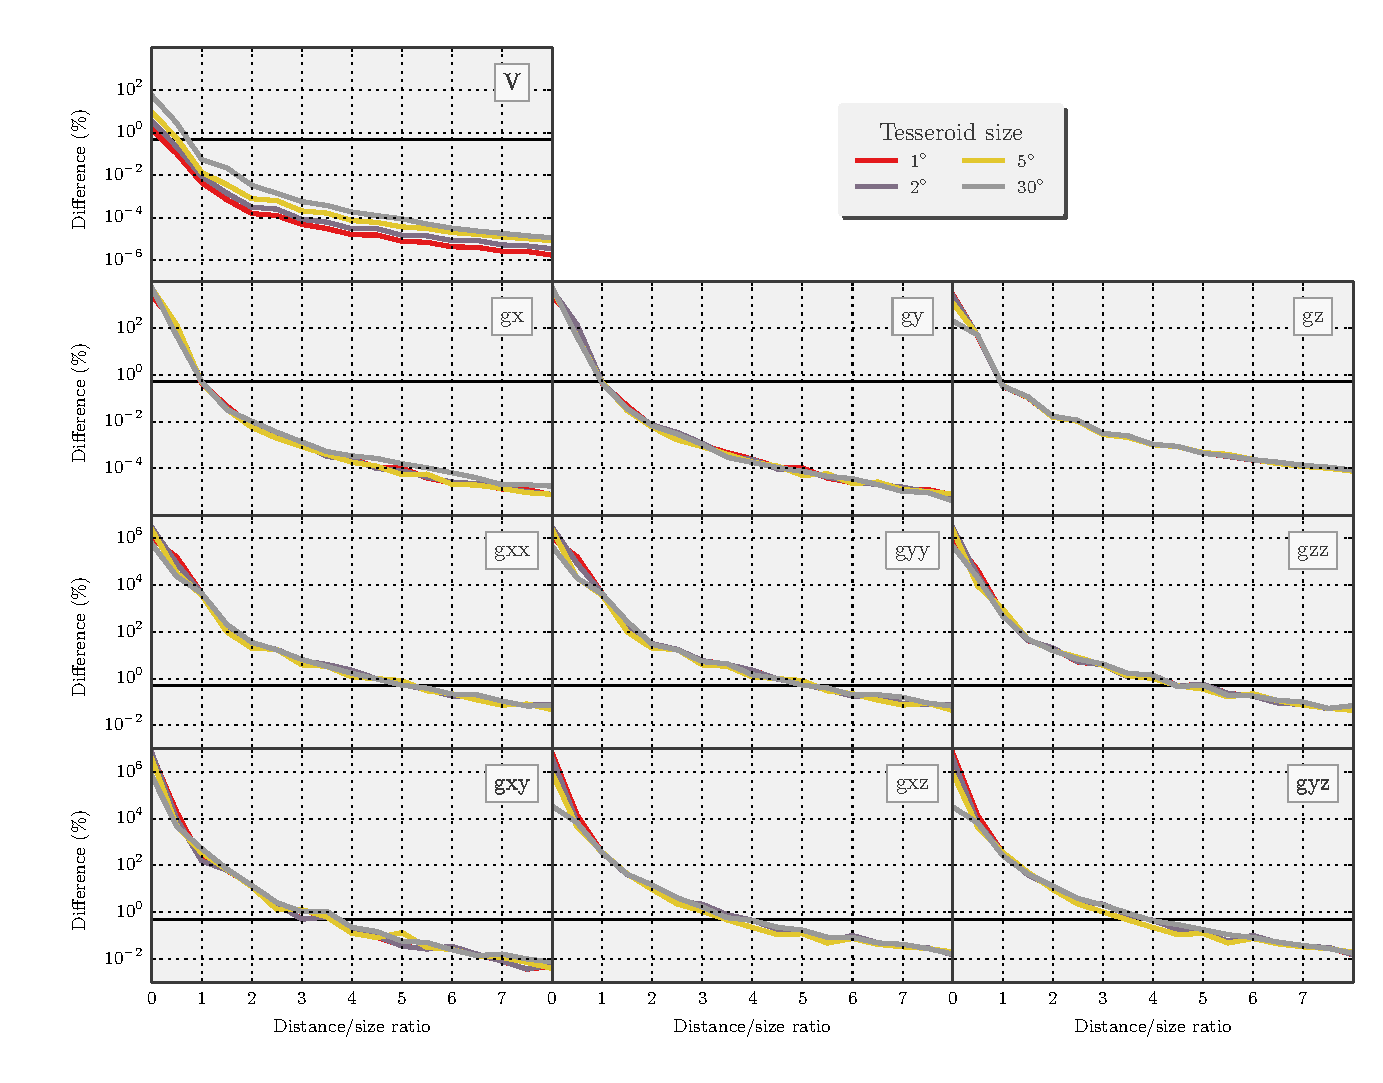
\includegraphics[width=\textwidth]{figs/tesseroid-x-shell}
    \caption{
        Tesseroid vs spherical shell.
    }
    \label{fig:tesseroid-x-shell}
\end{figure*}

%%%%%%%%%%%%%%%%%%%%%%%%%%%%%%%%%%%%%%%%%%%%%%%%%%%%%%%%%%%%%%%%%%%%%%%%%%%%%%
\section{Discussion}

%%%%%%%%%%%%%%%%%%%%%%%%%%%%%%%%%%%%%%%%%%%%%%%%%%%%%%%%%%%%%%%%%%%%%%%%%%%%%%
\section{Conclusions}

%%%%%%%%%%%%%%%%%%%%%%%%%%%%%%%%%%%%%%%%%%%%%%%%%%%%%%%%%%%%%%%%%%%%%%%%%%%%%%
\section{Acknowledgments}

Lorem ipsum dolor sit amet, consectetur adipiscing elit. Nam eu dolor pretium,
egestas mauris sed, dapibus quam. Duis hendrerit mollis nunc a consequat. Nulla
et sem consectetur, interdum velit eget, aliquam ipsum. Praesent sagittis
tortor diam, sed ultrices magna ullamcorper vitae. Proin vitae orci augue.
Morbi dictum ligula gravida sem malesuada facilisis. Mauris nibh metus, cursus
eget imperdiet vitae, pretium at lorem. Praesent nisi mauris, pretium ut risus
fermentum, egestas tincidunt nibh. Mauris nulla orci, consequat eu pharetra
non, mattis ut urna. Mauris facilisis orci eros. Nam mattis non magna iaculis
consectetur. Morbi sodales dolor vitae felis sagittis, eget faucibus turpis
convallis. Nullam malesuada, mauris et ultricies rutrum, odio nulla gravida
nunc, ac volutpat eros lectus eget lacus. Integer venenatis velit vel justo
pellentesque, quis molestie sem vestibulum.

\bibliographystyle{gji}
\bibliography{references}

\end{document}
